\chapter{Intelligence as an Operating System}

Most of what people call intelligence is not fixed at birth.

Some differences may be natural. There is no need to deny that. But the practical part of intelligence, the part that changes decisions, solves problems, earns trust, builds capital, and improves a life, is largely acquired. It is learned through concepts, corrected through action, and strengthened through repeated use.

A useful definition is:

\begin{quote}
Intelligence is the ability to solve problems.
\end{quote}

This does not mean solving every problem immediately. A person who can work on a hard problem for years, keep improving his method, and eventually solve it is showing a high form of intelligence. Patience, method, and correction are not outside intelligence. They are part of it.

So when you are tempted to say, ``My intelligence is not enough,'' add one word:

\begin{quote}
My intelligence is not enough yet.
\end{quote}

That word protects the future.

\section*{Concepts and Connections}

In this book, intelligence has already appeared under another name. It is the quality of a person's internal operating system.

At the base are concepts. But concepts alone are not enough. A mind full of isolated words is like a warehouse full of unassembled parts. The power comes from clear, accurate, necessary concepts and clear, accurate, necessary connections among them.

\begin{center}
\begin{adjustbox}{max width=\linewidth}
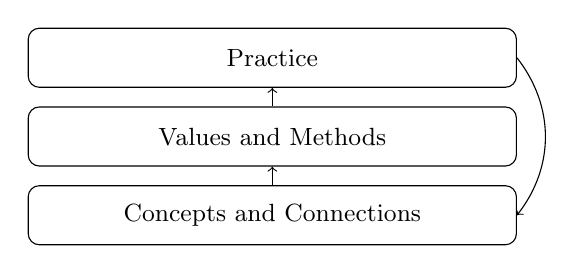
\begin{tikzpicture}[every node/.style={font=\small, align=center}]
\node[draw, rounded corners, minimum width=6.2cm, minimum height=0.75cm] (practice) at (0,2.0) {Practice};
\node[draw, rounded corners, minimum width=6.2cm, minimum height=0.75cm] (values) at (0,1.0) {Values and Methods};
\node[draw, rounded corners, minimum width=6.2cm, minimum height=0.75cm] (concepts) at (0,0) {Concepts and Connections};
\draw[->] (concepts) -- (values);
\draw[->] (values) -- (practice);
\draw[->, bend left=38] (practice.east) to (concepts.east);
\end{tikzpicture}
\end{adjustbox}
\end{center}

A new concept creates the possibility of higher intelligence. But the possibility becomes real only when the concept is used. If nothing changes in choice, action, attention, or review, then the concept has not yet entered the operating system. It is only a phrase remembered by the mouth.

This is why action matters so much. Some people act, review, adjust, and act again. Their intelligence rises through use. Others collect statements, admire them, and continue living as before. Their intelligence remains near its original level. Relative to a rising world, even standing still becomes falling behind.

\section*{Wrong Concepts Are Expensive}

Not knowing is dangerous. Not knowing that you do not know is worse. But there is an even more damaging condition: holding a wrong concept with confidence.

A missing concept leaves a blank. A wrong concept installs a bad instruction. If you then act diligently under that bad instruction, effort increases the damage.

Consider ``long term.'' Many people suffer because this concept is absent from their operating system. They judge usefulness only by immediate reward, so they ignore skills and knowledge that need years to show their value. But even when the phrase ``long term'' exists in the mind, it may not be connected correctly.

If ``long term'' is not connected to ``useful,'' a person may reject useful knowledge too early.

If ``long term'' is not connected to ``investing,'' a person may confuse market movement with decision quality.

If ``long term'' is not connected to ``writing,'' a person may quit after the first awkward pages.

The same problem appears with ``fragmentation.'' Many people connect fragmentation to learning and conclude that fragmented learning is useless. The better connection is different: time may be fragmented, but learning should remain continuous. Fifteen minutes a day can still belong to one coherent thread.

Or consider ``speed.'' Speed should not be connected to success in the childish form of ``quick success.'' Success usually needs time. But speed can be connected to entry. A person should often enter a field quickly, build the first rough map quickly, and reach the point where real practice can begin. Slow entry keeps people forever outside the door.

Intelligence improves when concepts are not only added, but reconnected.

\section*{Values and Methods}

Above concepts and connections sit two operating layers:

\begin{enumerate}
\item values;
\item methods.
\end{enumerate}

Values ask, ``What is better? What is best?''

Methods ask, ``How should this be done? How can this be improved?''

Values determine the quality of choice. Methods determine the quality of action after choice. Since choice is one of the central events of a life, and action is the material from which a life is made, these two layers are not decorative. They are decisive.

A person who has accepted that attention is more valuable than time, and time more valuable than money, begins to choose differently. He pays less attention to noise. He becomes less interested in hot news that changes nothing. He starts asking whether a book, project, conversation, or job deserves his best mental energy.

That is not merely a new opinion. It is intelligence in motion. A concept changed a value. A value changed a choice. A choice changed action. Action changed life.

\section*{Learning Must Become Use}

Growth often happens in small, traceable steps. Yesterday something was unclear. Today it becomes slightly clearer. Tomorrow a new connection appears. These moments deserve attention because they show the operating system upgrading itself.

But the upgrade is never completed by reading alone.

To learn a concept and not use it is like buying a tool and never taking it out of the box. The tool may be excellent, but the work remains undone. Many people give up before they experience the reward of applied learning. Then they explain the failure by saying intelligence is natural and effort is useless.

The explanation is convenient, but false in the useful sense.

Writing is a good example. Many people refuse to write because they think they do not write well. But almost nobody writes well at the beginning. People who become known for writing usually spend years, sometimes more than a decade, writing badly, then less badly, then clearly, then powerfully.

If your purpose is to clarify thinking, record experience, teach, persuade, or build a public surface for your ability, the first focus should not be ``write beautifully.'' The first focus should be ``continue writing and improve.'' Beauty may arrive later. Clarity may arrive through repetition. But nothing arrives if the work never begins.

\section*{Adjusting the Focus}

There is a practical shortcut for raising intelligence:

\begin{quote}
Adjust the focus of attention.
\end{quote}

The same object can produce different results depending on where attention rests. A beginner sees the obvious surface. A trained person sees structure, cause, missing conditions, and future consequences. The object did not change. The focus changed.

Book selection is a simple but important example.

Many people choose books by cover, title, celebrity recommendation, marketing band, price, or thickness. They think they are buying knowledge, but often they are buying paper, packaging, and social proof. A person serious about learning must put attention elsewhere.

For nonfiction books, more useful signals include:

\begin{enumerate}
\item edition history;
\item number of printings;
\item publisher quality;
\item reference list;
\item respect for primary sources.
\end{enumerate}

None of these signals is perfect. A frequently reprinted book can still be shallow. A serious book can have a plain cover. But these signals are closer to the real question: does this book deserve entry into my mind?

Buying the wrong object wastes money. Reading the wrong book can pollute judgment. Money can be earned again more easily than a damaged operating system can be repaired.

This is why attention saved from noise must not be left idle. It must be placed on better focal points.

\section*{A Focus Test}

Adjusting focus is not guesswork. It can be practiced as a method.

\begin{enumerate}
\item Look at the object, decision, or task from the current focus.
\item Ask what value judgment is hidden inside that focus.
\item Move the focus to another possible value.
\item Predict what choice this new focus would produce.
\item Compare the likely long-term consequences.
\item Keep the focus that produces better long-term results.
\end{enumerate}

This is metacognition applied to values. You are not merely thinking. You are watching how your thinking selects what to notice.

\begin{center}
\begin{adjustbox}{max width=\linewidth}
\begin{tikzpicture}[node distance=0.9cm, every node/.style={font=\small, align=center}]
\node[draw, rounded corners, minimum width=2.3cm, minimum height=0.75cm] (focus) {Focus};
\node[draw, rounded corners, minimum width=2.3cm, minimum height=0.75cm, right=of focus] (value) {Value};
\node[draw, rounded corners, minimum width=2.3cm, minimum height=0.75cm, right=of value] (choice) {Choice};
\node[draw, rounded corners, minimum width=2.3cm, minimum height=0.75cm, below=of value] (result) {Result};
\draw[->] (focus) -- (value);
\draw[->] (value) -- (choice);
\draw[->] (choice) |- (result);
\draw[->] (result) -| (focus);
\end{tikzpicture}
\end{adjustbox}
\end{center}

Over time, this practice becomes faster. At first, someone may need to tell you, ``You are looking at the wrong thing.'' Later, you can ask for yourself, ``How do I know which thing deserves attention?'' When you can answer that question with reasons, you can teach others.

\section*{Seeing Through Other Eyes}

One of the fastest ways to improve problem-solving ability is to move attention away from the self and into the viewpoint of another person.

Teaching makes this necessity visible. A teacher who only asks, ``How do I understand this?'' will fail many students. A better teacher asks:

\begin{quote}
What does this problem look like to the student?
\end{quote}

If the students can be sorted into several types, the next question is:

\begin{quote}
What does each type see, miss, fear, or misunderstand?
\end{quote}

The quality of teaching can be judged by whether different kinds of students can reach the same understanding through the teacher's guidance. This requires constant focus adjustment. The teacher must stop staring at his own clarity and investigate the student's confusion.

At first this feels impossible. How can one know what another person is thinking? But repeated practice changes the answer. Facial expression, timing, questions, silence, and wrong answers all become evidence. The teacher gradually learns to infer the hidden obstacle.

This method is not limited to classrooms. Writing requires the same skill. Sales requires it. Management requires it. Product design requires it. Negotiation requires it. Friendship and family life require it.

Many people call this emotional intelligence. The label is optional. In the framework of this book, it is simply intelligence applied to human problems.

\section*{Human Problems Are Still Problems}

If intelligence is problem-solving ability, then so-called emotional intelligence is the ability to solve problems involving people.

A person with poor interpersonal judgment often treats others as objects: fixed, mechanical, and simple. But people have motives, desires, fears, memories, expectations, emotions, and changing interpretations. To ignore these facts is not honesty. It is poor modeling.

A useful person models other people more accurately.

This connects directly to wealth freedom. Many people ask how to make money. A durable answer is:

\begin{quote}
Become useful to others.
\end{quote}

Doing something that pleases only yourself may be easy. Doing something that solves another person's problem, respects his situation, and is valuable enough for him to pay for is harder. But that is where exchange begins. Wealth is not created by staring at one's own desire. It is created by serving demand, reducing friction, solving problems, and earning trust.

So the habit of seeing through other eyes is not merely kindness. It is productive intelligence.

\section*{Only Better, Not Best}

There is one anxiety hidden inside focus adjustment: what if there is an even better focus?

There usually is.

In the long term, there is almost always a better method, better concept, better connection, better tool, better question, or better strategy. If there were a final best, human development would have stopped long ago.

This does not mean current action is foolish. It means the current choice must be treated properly.

Short term may contain a best-known choice. Long term contains only better choices.

\begin{quote}
The best available choice now is not invalidated by the possibility of a better choice later.
\end{quote}

If you refuse to act until perfect safety appears, you will not become safer. You will become motionless. Many people search for one hundred percent certainty in domains where such certainty cannot exist. Then they wonder why life has not changed.

The method is more practical:

\begin{enumerate}
\item choose the best focus you can justify now;
\item act under that focus;
\item observe the result;
\item revise when evidence demands revision.
\end{enumerate}

Without action, you cannot even discover what the better focus might be. Practice supplies evidence that imagination cannot.

\section*{The Upgrade Loop}

The operating system of intelligence upgrades through a loop.

\begin{center}
\begin{adjustbox}{max width=\linewidth}
\begin{tikzpicture}[node distance=1.0cm, every node/.style={font=\small, align=center}]
\node[draw, rounded corners, minimum width=2.5cm, minimum height=0.75cm] (concept) {Concept};
\node[draw, rounded corners, minimum width=2.5cm, minimum height=0.75cm, right=of concept] (link) {Connection};
\node[draw, rounded corners, minimum width=2.5cm, minimum height=0.75cm, right=of link] (value) {Value};
\node[draw, rounded corners, minimum width=2.5cm, minimum height=0.75cm, below=of link] (method) {Method};
\node[draw, rounded corners, minimum width=2.5cm, minimum height=0.75cm, left=of method] (action) {Practice};
\node[draw, rounded corners, minimum width=2.5cm, minimum height=0.75cm, right=of method] (review) {Review};
\draw[->] (concept) -- (link);
\draw[->] (link) -- (value);
\draw[->] (value) |- (method);
\draw[->] (method) -- (action);
\draw[->] (action) -- (review);
\draw[->] (review) -| (concept);
\end{tikzpicture}
\end{adjustbox}
\end{center}

A person learns a concept, builds connections, updates values, forms methods, practices, reviews, and then revises the concept again. This is not mysterious. It is the ordinary machinery of growth made visible.

The earlier chapters of this book have all been installing parts of this machinery. Attention taught us what must be protected. Long-term thinking taught us how value appears over time. Knowledge taught us how information becomes useful. Growth rate taught us to care not only about improvement, but about the rate of improvement. Writing taught us to clarify thought through production. Choice taught us to add necessary conditions.

This chapter gives the machinery a name: practical intelligence.

\section*{A Pocket Checklist}

When facing a decision, a book, a project, a person, or a problem, use this short checklist:

\begin{enumerate}
\item What concept am I using here?
\item Is the concept clear, accurate, and necessary?
\item What other concepts should it be connected to?
\item What value judgment is guiding my attention?
\item What method follows from that value?
\item What would this look like from another person's position?
\item What action can test the current focus?
\item What result would make me revise?
\end{enumerate}

This checklist is not a ritual. It is a way to keep the operating system awake.

The goal is not to appear intelligent. The goal is to solve better problems, make better choices, become more useful, and keep upgrading. In the practice of wealth freedom, intelligence is not a score. It is a living system: concepts connected well, values chosen carefully, methods improved repeatedly, and action used as the final test.
